\section{Data Preparation}

Cleaning is a critical step in any data analysis pipeline. Think of it as preparing a field before planting .We remove the weeds, till the soil, and make sure everything is ready for growth. Similarly, we clean our dataset to remove inconsistencies and get it analysis-ready.

\subsection*{Loading Dataset}
To load the agricultural dataset into R, we use the following command:

\begin{verbatim}
data_agri <- read.csv("/content/agriculture.csv")
\end{verbatim}

\subsection*{Data Inspection}
With the agricultural dataset already loaded into \texttt{data\_agri}, our next step is to inspect its structure and identify any data quality issues. This inspection helps us understand what kind of cleaning might be necessary before merging it with the climate dataset. We use the following commands to explore the dataset:

\begin{verbatim}
glimpse(data_agri)
\end{verbatim}

% Figure here-----------------------------
\begin{figure}[h]
\centering
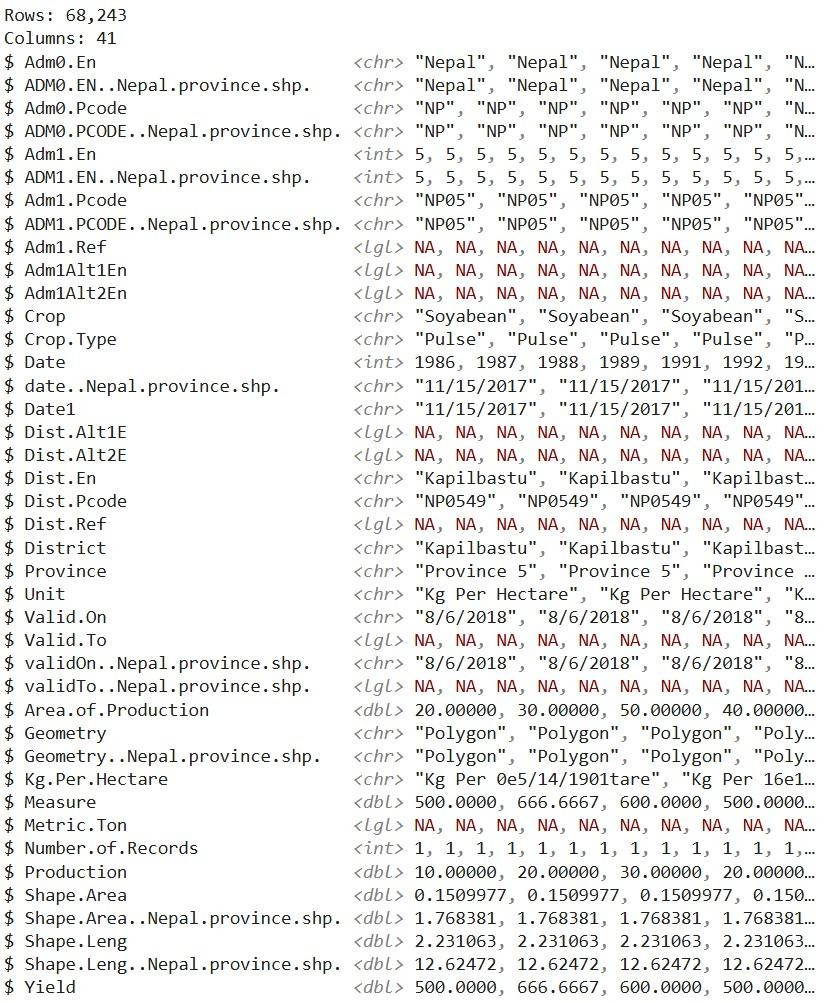
\includegraphics[width=0.6\textwidth]{figures/agri_glimpse.jpg}
\caption{Glimpse of Agricultural Dataset}
\end{figure}

\subsection*{Data Cleaning}
\subsubsection*{Checking for Missing Values}
The next step is checking for missing values in the dataset to understand the completeness of the data.

\begin{verbatim}
sum(is.na(data_agri))          # Total missing values
colSums(is.na(data_agri))      # Missing values per column
\end{verbatim}

% Figure here------------------------
\begin{figure}[h]
\centering
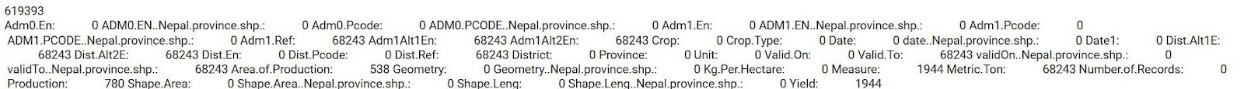
\includegraphics[width=0.8\textwidth]{figures/missing_data_agri.jpg}
\caption{Missing data information
}

\end{figure}

\textbf{Explanation of each function:}
\begin{itemize}
    \item \texttt{glimpse(data\_agri)}: Offers a compact view of the dataset, showing each column’s name, data type, and a preview of its values.
    \item \texttt{sum(is.na(data\_agri))}: Displays the total count of missing values across the entire dataset.
    \item \texttt{colSums(is.na(data\_agri))}: Shows the number of missing entries in each column individually, helping us pinpoint where problems lie.
\end{itemize}

This step is crucial for understanding the completeness and structure of the data. Based on these results, we’ll decide which cleaning operations are necessary to prepare the dataset for merging with the climate records.

\subsubsection*{Dropping Unwanted Columns}
Based on our inspection, we identified several metadata and geometry-related columns in the agricultural dataset that are not relevant for our analysis. These include administrative codes, geometry information, shape metrics, and other auxiliary fields. To streamline our dataset and retain only meaningful columns, we define a list of columns to drop and then use the \texttt{dplyr::select()} function to remove them:

\begin{verbatim}
columns_to_drop <- c(
  "Adm0.En", "ADM0.EN..Nepal.province.shp.", "Adm0.Pcode",
  "ADM0.PCODE..Nepal.province.shp.","Adm1.En", "ADM1.EN..Nepal.province.shp.",
   "Adm1.Pcode","ADM1.PCODE..Nepal.province.shp.",
  "Adm1.Ref", "Adm1Alt1En", "Adm1Alt2En", "date..Nepal.province.shp.", "Date1",
  "Dist.Alt1E", "Dist.Alt2E", "Dist.En", "Dist.Pcode", "Dist.Ref","Unit", 
  "Valid.On", "Valid.To", "validOn..Nepal.province.shp.", 
  "validTo..Nepal.province.shp.","Area.of.Production", "Geometry", 
  "Geometry..Nepal.province.shp.","Kg.Per.Hectare", "Measure", "Metric.Ton", 
  "Number.of.Records","Shape.Area", "Shape.Area..Nepal.province.shp.", 
  "Shape.Leng", "Shape.Leng..Nepal.province.shp."
)

data_agri_clean <- data_agri %>%
  select(-all_of(columns_to_drop))
\end{verbatim}

This command creates a new cleaned version of the dataset, \texttt{data\_agri\_clean}, which contains only the essential information for further analysis and integration with the climate data.

\begin{verbatim}
data_agri_clean <- data_agri_clean %>%
  rename(Year = Date)
\end{verbatim}
\clearpage
% Fugure here----------------------------
\begin{figure}[h]
\centering
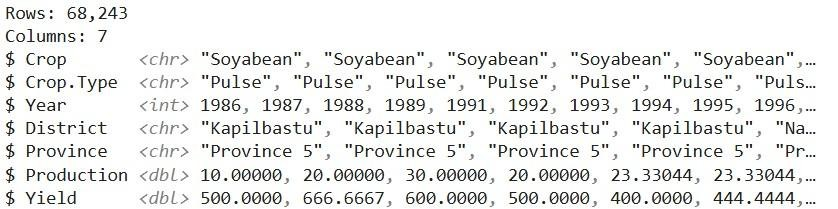
\includegraphics[width=0.6\textwidth]{figures/cleaned_agri.jpg}
\caption{ Glimpse of Agricultural Dataset after cleaning}
\end{figure}

\begin{verbatim}
summary(data_agri_clean)
\end{verbatim}

% Figure here--------------------------
\begin{figure}[h]
\centering
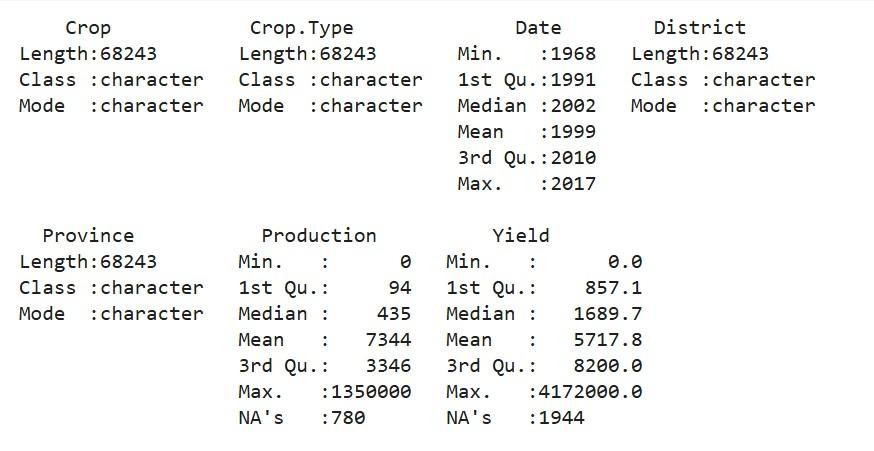
\includegraphics[width=0.6\textwidth]{figures/summary_agri.jpg}
\caption{ Summary of Agricultural Dataset after cleaning}
\end{figure}

When you’re working with data, it’s like putting together a giant puzzle. Sometimes, pieces of that puzzle go missing.

\subsubsection*{Analysis of the Production and Yield Variables}
Both the \texttt{Production} and \texttt{Yield} variables in the agricultural dataset exhibit missing values and considerable skewness due to extreme outliers. A careful examination of their distributions is necessary to determine the most appropriate imputation strategies.

\subsubsection*{Missing Data Overview}
\begin{itemize}
    \item \textbf{Production:} Contains 1972 missing values out of 68,243 records (approximately 2.89\%).
    \item \textbf{Yield:} Contains 1944 missing values out of 68,243 records (approximately 2.85\%).
\end{itemize}

\textbf{Summary statistics of Yield with and without outliers:}
\begin{verbatim}
summary(data_agri_clean$Yield)
\end{verbatim}
\begin{verbatim}
clean_yield <- data_agri_clean %>% 
filter(Yield >= lower_bound & Yield <= upper_bound)
summary(clean_yield$Yield)
\end{verbatim}

% Figure here----------------------------
\begin{figure}[h]
\centering
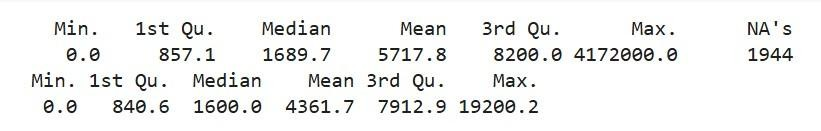
\includegraphics[width=0.6\textwidth]{figures/summary_yield.jpg}
\caption{Summary of Yield with and without Outliers}
\end{figure}

\subsubsection*{Summary statistics of Production with and without outliers:}
\begin{verbatim}
summary(data_agri_clean$Production)
\end{verbatim}

\begin{verbatim}
clean_production <- data_agri_clean %>% 
filter(Production >= lower_bound & Production <= upper_bound)
summary(clean_production$Production)
\end{verbatim}

% Figure here---------------------------
\begin{figure}[h]
\centering
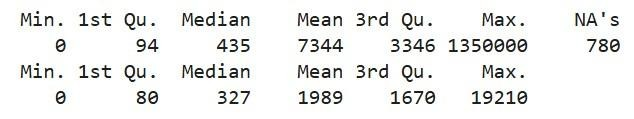
\includegraphics[width=0.5\textwidth]{figures/summ_prod.jpg}
\caption{Summary of Production with and without Outliers}
\end{figure}

The analysis of both \texttt{Yield} and \texttt{Production} variables highlights significant skewness and the presence of extreme outliers in the raw data:
\begin{itemize}
    \item For \texttt{Yield}, the maximum value drops dramatically from 4,172,000.0 to 19,200.2 after outlier removal, with the mean decreasing from 5717.8 to 4361.7, and the median shifting slightly from 1689.7 to 1600.0. This confirms a strong right-skew even in the cleaned data.
    \item For \texttt{Production}, the maximum drops from 1,350,000 to 19,210, and the mean declines sharply from 7344 to 1989, while the median drops from 435 to 327. This further confirms the influence of extreme values in inflating central tendencies.
\end{itemize}

These patterns confirm that both variables are not normally distributed and are heavily affected by extreme values. The contrast between the mean and median, especially in the original data, reinforces the appropriateness of using the median as an imputation strategy for missing values. It provides a robust and representative estimate of central tendency that is not skewed by a few extreme values.
Moreover, the percentage of missing data is $2.85\%$ for Yield and $1.14\%$ for Production  is low enough to justify imputation over deletion, ensuring the retention of valuable information while maintaining the dataset’s integrity.
\textbf{Hence, median imputation will be applied to both variables using the median calculated from the dataset after outlier removal.} This approach prepares the dataset for merging with climate data in a way that is statistically sound and analytically reliable.

\subsubsection*{Median Imputation for Missing Values}

\textbf{What is Median Imputation?}\\
Median imputation is a statistical technique used to handle missing values in a dataset by replacing them with the median of the observed (non-missing) values in the same variable. The median represents the middle value of a sorted dataset and is less sensitive to extreme values (outliers) compared to the mean.

\textbf{Why Use Median Imputation?}\\
In our dataset, both \texttt{Production} and \texttt{Yield} variables exhibit strong right-skewed distributions with significant outliers. Under such conditions, using the mean for imputation would inflate the imputed values and distort the dataset. Instead, median imputation provides a more robust and representative central value.

\begin{itemize}
    \item \textbf{Resilience to Outliers:} The median is not affected by very large or very small values, making it ideal for skewed data.
    \item \textbf{Preserves Distributional Shape:} Median imputation helps maintain the original shape and spread of the variable’s distribution.
    \item \textbf{Minimal Data Loss:} This method allows us to retain all observations, ensuring the dataset remains as complete as possible.
\end{itemize}

\textbf{Application in Our Dataset}\\
We observed missing values in both variables:
\begin{itemize}
    \item \texttt{Yield:} 1944 missing values (2.85\% of total observations)
    \item \texttt{Production:} 780 missing values (1.14\% of total observations)
\end{itemize}

Due to the low proportion of missingness and the skewed distributions, we impute the missing values using the median computed from the cleaned (outlier-removed) dataset:

\begin{verbatim}
median_yield <- median(data_agri_clean$Yield, na.rm = TRUE)
data_agri_clean$Yield[is.na(data_agri_clean$Yield)] <- median_yield
sum(is.na(data_agri_clean$Yield))
summary(data_agri_clean$Yield)
\end{verbatim}

% Figure here-----------------------------
\begin{figure}[h]
\centering
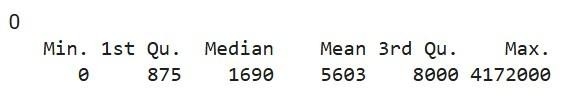
\includegraphics[width=0.5\textwidth]{figures/impute_yield.jpg}
\caption{ Summary of Yield after imputation}
\end{figure}

\begin{verbatim}
median_production <- median(data_agri_clean$Production, na.rm = TRUE)
data_agri_clean$Production[is.na(data_agri_clean$Production)] <-
median_production
sum(is.na(data_agri_clean$Production))
summary(data_agri_clean$Production)
\end{verbatim}

% Figur here----------------------------
\begin{figure}[h]
\centering
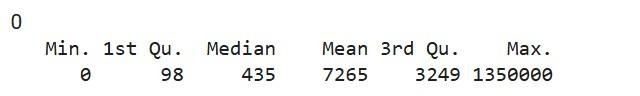
\includegraphics[width=0.5\textwidth]{figures/impute_prod.jpg}
\caption{ Summary of Production after imputation}
\end{figure}

